%https://www.overleaf.com/7690515vynnjrmjmtvc#/26945709/
\documentclass[
12pt,
a4paper,
BCOR10mm,
%chapterprefix,
DIV14,
headsepline,
%twoside,
%openright
]{scrreprt}

\KOMAoptions{
	listof=totoc,
	bibliography=totoc,
	index=totoc
}

\usepackage[T1]{fontenc}
\usepackage[utf8]{inputenc}

\usepackage{lmodern}

\usepackage[ngerman,english]{babel}

\usepackage[toc]{appendix}
\usepackage{eurosym}
\usepackage{fancyhdr}
\usepackage{graphicx}
\usepackage[htt]{hyphenat}
\usepackage{listings}
\usepackage{amsmath}
\usepackage{microtype}
\usepackage[list=true,hypcap=true]{subcaption}
\usepackage{units}
\usepackage{tikz}
\usepackage{pgfplots}
\usepackage{pgfplotstable}
\usepackage{float}
\usepackage{graphicx}
\usepackage{filecontents}
\usepackage{varioref}
\usepackage[hidelinks]{hyperref}
\usepackage[capitalise,noabbrev]{cleveref}

\lstset{
	basicstyle=\ttfamily,
	frame=single,
	numbers=left,
	language=C,
	breaklines=true,
	breakatwhitespace=true,
	postbreak=\hbox{$\hookrightarrow$ },
	showstringspaces=false,
	tabsize=4,
	captionpos=b,
	morekeywords={gboolean,gpointer,gconstpointer,gchar,guchar,gint,guint,gshort,gushort,glong,gulong,gint8,guint8,gint16,guint16,gint32,guint32,gint64,guint64,gfloat,gdouble,gsize,gssize,goffset,gintptr,guintptr,int8_t,uint8_t,int16_t,uint16_t,int32_t,uint32_t,int64_t,uint64_t,size_t,ssize_t,off_t,intptr_t,uintptr_t,mode_t}
}

\makeatletter
\renewcommand*{\lstlistlistingname}{List of Listings}
\makeatother

\begin{document}
	
	\begin{titlepage}
		\begin{center}
			{\titlefont\huge Programmieren einer Simulation für kurzreichweitige Partikel Interaktionen\par}
			
			\bigskip
			\bigskip
			
			{\Large Projektbericht\par}
			
			\bigskip
			\bigskip
			
			{\large Arbeitsbereich Wissenschaftliches Rechnen\\
				Fachbereich Informatik\\
				Fakultät für Mathematik, Informatik und Naturwissenschaften\\
				Universität Hamburg\par}
		\end{center}
		
		\vfill
		
		{\large\begin{tabular}{ll}
				Vorgelegt von:  & \begin{tabular}{@{}l@{}}Oliver Heidmann (6420331), \\ Benjamin Warnke (6676867)\end{tabular} \\
				E-Mail-Adresse: & \begin{tabular}{@{}l@{}}\href{mailto:oliverheidmann@hotmail.de}{oliverheidmann@hotmail.de},\\ \href{mailto:4bwarnke@informatik.uni-hamburg.de}{4bwarnke@informatik.uni-hamburg.de}\end{tabular}\\
				Studiengang:    &Bachelor Software System Entwicklung\\ & Bachelor Informatik\\
				\\
				Betreuer:       & Philipp Neumann \\
				\\
				Hamburg, den 09.03.2017
			\end{tabular}\par}
	\end{titlepage}
	
	\chapter*{Abstrakt}%DONE
	\thispagestyle{empty}
	Ziel des Projektes ist die Implementierung einer Partikel Simulation für kurzreichweitige Interaktionen, mit automatischer Auswahl der am besten wirkenden Optimierung für die gegebenen Eingabedaten.
	\tableofcontents
	
	\chapter{Einleitung}%DONE
	\label{Einleitung}
	Bei Partikel Simulationen müssen in der naiven Implementation die Wechselwirkungen zwischen jedem möglichen Partikelpaar berechnet werden. Die Laufzeit des Programms steigt quadratisch zur Anzahl der Partikel. Dies ist besonders bei hohen Anzahlen von Partikeln kritisch für die Laufzeit. Die in diesem Projekt implementierte Partikel-Simulation ist für kurzreichweitige Interaktionen optimiert. Dadurch lassen sich die Interaktionen zwischen weit auseinanderliegenden Partikeln vernachlässigen, wodurch die Laufzeit kürzer werden kann. Es gibt verschiedene Möglichkeiten, die Interaktionen auf die kurzreichweitige Interaktion zu beschränken um das Programm zu beschleunigen. Das Problem bei diesen verschiedenen Möglichkeiten der Beschleunigung besteht darin, dass je nach Eingabe eine andere Art der Vereinfachung eine bessere Programm-Laufzeit ermöglicht. Die Besonderheit dieser Partikel Simulation liegt darin, dass das Programm zu beginn selbst entscheiden kann, welche Optimierungsstrategie für die gegebene Eingabe am sinnvollsten ist. Dies ist besonders dann spannend, wenn fraglich ist, welches Verfahren für die Eingabe am besten geeignet ist, ohne vorher alle Möglichkeiten auszuprobieren.
	
	\chapter{Aufgabenstellung}%DONE
	\label{Aufgabenstellung}
	Die Aufgabe für dieses Projekt bestand darin, eine Partikel-Simulation für kurzreichweitige Partikel Interaktionen zu schreiben. Im Zusammenspiel mit den kurzreichweitigen Interaktionen gibt es verschiedene Ansätze die Laufzeit zu verringern. Einer der Ansätze besteht darin, eine Zellenstruktur zu definieren, die den Raum in kleinere Bereiche unterteilt. Ein anderer Ansatz basiert darauf, dass die Nachbarschaftsverhältnisse einmalig berechnet werden, und später mehrfach wiederverwendet werden können, da sich die Nachbarschaft selten ändert. Es ist möglich beide Varianten zu einer dritten zu kombinieren. Teil der Aufgabenstellung war es die eben genannten Ansätze zu implementieren. Der zentrale Kern der Aufgabenstellung bezieht sich auf die automatische Auswahl der schnellsten Variante unter Berücksichtigung der aktuellen Optionen. Dies wird im folgenden als Auto-Tuning bezeichnet. Für die Interaktionen zwischen Partikeln soll das Lennard-Jones Potential verwendet werden, dies soll für spätere Erweiterungen austauschbar sein. Um eine hohe Laufzeiteffizienz zu erreichen sollte eine Compilersprache wie Fortran oder C/Cpp verwendet werden. Aufgrund der Hardwarenähe haben wir uns dazu entschieden Cpp zu verwenden. Dies ermöglicht es mithilfe von OpenMP das Programm zu parallelisieren. Zusätzlich können die Vektorisierungsmöglichkeiten des Compilers genutzt werden. Die Simulation soll mit verschiedenartigen Eingaben starten können. Zum einen soll es möglich sein, die Startdaten aus einer Datei zu laden, zum anderen soll es auch relativ einfach möglich sein Daten nach vorgegebenen Mustern zu generieren, um Interaktionen darauf basierend berechnen zu können. Während und nach der Simulation sollen die Partikel Positionen abgespeichert werden, damit diese für spätere Analysen verwendet werden können. Um große Volumen zu Simulieren ist es sinnvoll, periodische Ränder zu verwenden, bei denen die Partikel auch über die Grenzen des Raumes hinweg miteinander Interagieren. Dies ermöglicht es einen Ausschnitt eines sehr großen Bereichs zu simulieren, und dadurch auf das Verhalten in einem größeren Kontext zu schließen. Als Literatur sollen die Quellen \cite{NumerischeSimulationInDerMolekuldynamic} und \cite{DCRapaport} gelesen werden.
	\chapter{Grundkonzepte}%DONE
	\label{Grundkonzepte}
	Im folgenden werden die in der Simulation verwendeten Grundkonzepte beschrieben. Sie bilden sowohl die Grundlage des Designs als auch die Grundlage der Implementation.
	\section{Lennard-Jones-Potential}%DONE
	Das Lennard-Jones-Potential beschreibt die kurzreichweitige Interaktion zwischen zwei verschiedenen Partikeln. Es ist möglich mit diesem Verfahren auch Interaktionen zwischen Partikeln unterschiedlichen Typs zu berechnen. Das Potential liefert die Kraft welche zwischen zwei gegebenen Partikeln wirkt. Obwohl es nur eine Annäherung an die, aus der Quantenmechanik resultierenden Kräfte ist, sind die Abweichungen zur Realität klein genug um relevante Daten zu erhalten. Des weiteren ist der benötigte Rechenaufwand um ein vielfaches geringer und ermöglicht somit die Simulation mit einer hohen Anzahl von Partikeln. Deshalb wird diese Art der Modellierung sehr häufig für Partikel Simulationen benutzt, obwohl es genauere Verfahren gibt. Das Potential wird in dem Rapport \cite{DCRapaport} beschrieben. Auf Seite 12 der Quelle \cite{DCRapaport} befindet sich die folgende Formel:
	\begin{align*}
	f_{n,i,j}=&\left(\frac{48\epsilon_{i,j}}{\sigma_{i,j}^2}\right)\cdot\left[\left(\frac{\sigma_{i,j}}{r_{n,i,j}}\right)^{14}-\frac{1}{2}\left(\frac{\sigma_{i,j}}{r_{n,i,j}}\right)^8\right]\cdot r_{n,i,j}
	\end{align*}
	Der folgende Graph ist eine Visualisierung der vorherigen Formel. $\epsilon$ und $\sigma$ sind für die Visualisierung auf 1 gesetzt worden.
	\begin{figure}[h]
		\centering
		\begin{tikzpicture}
		\begin{axis}[
		width=0.5\textwidth,
		height=0.2\textheight,
		xmin = 0.5,
		xmax = 4,
		xtick = {1,1.5,...,3.5},
		ymin = -3.5,
		ymax = 3.5,
		ytick = {-3,...,3},
		xlabel = r, 
		ylabel = f]
		\addplot[domain=1:4, samples=1000]{(48/1)*((1/x)^14 - 0.5*(1/x)^8)};
		\end{axis}
		\end{tikzpicture}
		\caption{Lennard- Jones Graph}
		\label{figure:LennardJonesGraph}
	\end{figure}\\
	Sobald der Abstand $r$ kleiner ist als $1.25$ überwiegen die abstoßenden Kräfte zwischen den Partikeln. Sobald der Abstand kleiner wird als 1, würde dies bedeuten, dass die Partikel physikalisch überlappen. Dieser Fall kann in dieser Simulation nicht auftreten. Für $r$ größer als $1.25$ gilt, dass die anziehenden Kräfte überwiegen. Sobald der Abstand größer wird als 2, wirken zwar noch anziehende Kräfte, diese sind aber so gering, dass diese vernachlässigbar klein sind. An dieser Stelle setzen die folgenden Optimierungsstrategien an. Der Punkt, ab dem die Kraft zwischen anziehen und abstoßen umkippt, hängt von den Konstanten $\epsilon$ und $\sigma$ ab. Die Variablen $i$ und $j$ sind Indizes, welche zwei verschiedene Partikel eindeutig identifizieren.
	\section{Störmer-Verlet-Integration}%DONE
	Aufgrund der großen Partikel Anzahl ist es nicht möglich, eine geschlossene Formel für die Position eines Partikels zur Zeit t aufzustellen. Daher muss ein iteratives nummerisches Verfahren genutzt werden. Das Störmer-Verlet-Verfahren hängt nur von wenigen Variablen ab und der Rechenfehler gering. Deshalb wird dieses Verfahren in Bewegungs-Simulationen angewendet. In diesem Projekt wurde eine Variante der Integration verwendet, die nur von den Positionen der Partikel abhängt. Dies hat den Vorteil, dass nur wenige Daten gespeichert, kopiert und berechnet werden müssen. Dadurch wird die Laufzeit so kurz wie möglich gehalten. Die Formel für die Integration wurde in der Quelle \cite{VerletAlgorithmusWiki} erläutert. Die Formel ist:
	\begin{align*}
	\vec{x}_{1,i}&=\vec{x}_{0,i}+\vec{v}_{0,i}\Delta t+\frac{1}{2}\vec{a}_{0,i}\Delta t^2\\
	\vec{x}_{n+1,i}&=2\vec{x}_{n,i}-\vec{x}_{n-1,i}+\vec{a}_{n,i}\Delta t^2
	\end{align*}\\
	Da durch diese Art der Integration keine Daten über die Geschwindigkeit vorhanden sind, wird häufig der Velocity-Verlet Algorithmus oder die Leapfrog Methode angewendet. Wenn eine spätere Erweiterung Daten über die Geschwindigkeit braucht, dann muss entweder eine andere Art der Integration verwendet werden, oder die Geschwindigkeiten aus den Positionsänderungen herausgerechnet werden. Da das Lennard-Jones Potential nur die aktuellen Positionen benötigt, wurde in diesem Projekt nur der Störmer-Verlet-Algorithmus verwendet.
	\newpage
	\section{Linked-Cells}%DONE
	Bei dieser Methode die Partikel zu strukturieren wird der Raum in mehrere gleich große Zellen unterteilt. Anzahl und Größe der Zellen hängen von dem in der Simulation benutzten cut-off-Radius ab. Die Partikel werden nun aufgrund ihrer räumlichen Position in die jeweiligen Zellen einsortiert. Der cut-off-Radius definiert den Maximalabstand, bis zu dem die Partikel miteinander interagieren. Damit die Datenstruktur nicht jede Iteration neu organisiert werden muss, wird der cut-off- Radius um einen konstanten Faktor erweitert. Dieser Radius wird diesem Programm als Parameter übergeben. Die Aufteilung der Partikel auf verschiedene Zellen führt dazu, dass für die Berechnungen der Interaktionen nur ein Teil der Partikel Betrachtet werden muss. Genauer genommen müssen für die Berechnung der Partikel in einer Zelle nur 13 von 26 Nachbarzellen sowie die Partikel in der Zelle selbst betrachtet werden.
	\begin{figure}[h]
		\centering
		\includegraphics[width=0.6\textwidth]{LinkedCells_Zoom_1.png}
		\caption{Linked-Cells Struktur}
		\label{figure:LinkedCellsStructure}
	\end{figure}
	In der Figure \ref{figure:LinkedCellsStructure} kann man die eben genannten Aspekte sehen. Alle Partikel, die sich in dem grünen Kreis befinden, müssen mit dem einen vollständig gelb gefüllten Partikel interagieren. Die Datenstruktur sorgt nun dafür, dass nur die Nachbarzellen betrachtet werden. Diese Nachbarzellen sind in der Grafik rot markiert. Partikel, die sich in dem rot markierten Gebiet befinden, und nicht in dem grünen Kreis, werden unnötigerweise als Nachbarn betrachtet, und erst sehr spät als irrelevant verworfen. Partikel, die sich in dem weißen Bereich befinden, müssen während der Berechnung gar nicht betrachtet werden. Bei einer hohen Anzahl von Zellen befinden sich die meisten Partikel außerhalb der relevanten Reichweite, und führen zu einer Verkürzung der Programmlaufzeit im Vergleich zur naiven Implementierung. Dadurch, dass sich relativ wenig Partikel in der gleichen Zelle befinden, sind die Partikel, die sich in einer Zelle befinden nahe beieinander im Speicher. Dies führt zu einer deutlich höheren Cache-Treffer Rate, als in den anderen Varianten, welche keine räumliche Unterteilung vornehmen.
	\section{Verlet-Listen}%DONE
	Bei Verlet-Listen existiert für jedes Partikel eine Liste der Nachbarn. Die Nachbarn werden aufgrund der Nähe der Partikel in entsprechende Listen einsortiert. Bei der Berechnung der Interaktionen, wird auf die Liste der Nachbarn zurückgegriffen, und nur mit jenen Partikeln eine Berechnung durchgeführt. Zu Beginn der Simulation sowie alle $i$ Simulationsschritte müssen die Listen für jedes Partikel neu generiert werden, wobei jede Partikel Position mit allen anderen Positionen verglichen wird. Um die Neugenerierung der Listen möglichst selten auszuführen wird auf den cut-off- Radius genau wie bei der Linked-Cells Variante eine zusätzliche Distanz hinzugefügt. Je größer die zusätzliche Distanz ist, desto seltener müssen die Nachbarschaftslisten rekonstruiert werden. 
	Die Nachbarschaftslisten zu rekonstruieren braucht relativ viel Zeit, da alle möglichen Partikelkombinationen betrachtet werden müssen. Dies führt dazu, dass die Rekonstruktion eine quadratische Laufzeit hat. Zusätzlich haben die Verlet-Listen das Problem, dass die Partikel nicht nahe beieinander im Speicher liegen. Dies führt dazu, dass es zur wenige Cache Treffer gibt, wodurch die Laufzeit verlangsamt wird.
	\begin{figure}[h]
		\centering
		\includegraphics[width=0.6\textwidth]{VerletList_Zoom_1.png}
		\caption{Verlet-Listen Struktur}
		\label{figure:VerletListsStructure}
	\end{figure}
	In der Figure \ref{figure:VerletListsStructure} ist durch blaue Pfeile dargestellt, welche Partikelkombinationen auf Nachbarschaft getestet werden müssen, um die Liste des einen Partikels in der Mitte herausfinden zu können. Der Vorteil dieser Datenstruktur besteht darin, dass der rote Kreis kaum größer ist als der grüne Kreis. Dies bedeutet, dass während der Iterationen, in denen die Datenstruktur nicht rekonstruiert werden muss, die Laufzeit deutlich geringer ist, da kaum unnötige Partikelpaare betrachtet werden.
	\section{Linked-Cells + Verlet-Listen}%DONE
	Nachdem beide Datenstrukturen vorliegen, ist es einfach möglich, diese zu kombinieren, um die Vorteile zu verstärken, und die Nachteile zu verdecken. Von der Zellen basierten Variante nutzt man den Vorteil, dass Partikel, die im Raum nahe beieinander sind auch im Speicher nahe beieinander sind. Dies führt zu einer genauso hohen Cache Treffer Rate, wie bei der nur Zellen basierten Variante. Um die Rekonstruktion der Nachbarlisten zu beschleunigen nutzt man die Eigenschaft der Zellen, nach der benachbarte Partikel ausschließlich in benachbarten Zellen zu finden sind. Durch den zweistufigen Aufwand, die Nachbarn zu erkennen, wird für die Rekonstruierung der Datenstruktur mehr Zeit benötigt, als in der Zellen basierten Variante. Betrachtet man den Vergleich zwischen der kombinierten Variante und der nur Listen Variante, dann hat sich die Zeit zur Rekonstruktion deutlich verkürzt. Während der Berechnung der Interaktionen, ist diese Variante genau wie die Listen basierte Variante schneller, als die nur Zellen basierte Variante. Durch die Vereinigung von verschiedenen Vor- und Nachteilen, ist diese Optimierungsvariante manchmal schneller, als die nur Zellen basierte Variante, und gleichzeitig ist diese Variante immer schneller, als die nur Listen basierte Variante.
	\begin{figure}[h]
		\centering
		\includegraphics[width=0.6\textwidth]{LinkedCells_VerletList_Zoom_1.png}
		\caption{Linked-Cells+Verlet-Listen Struktur}
		\label{figure:LinkedCellsVerletListStructure}
	\end{figure}\\
	In der Figure \ref{figure:VerletListsStructure} kann man erkennen, dass durch die Kombination die Anzahl der blau markierten Nachbarschafts Tests zum Aufbau der Nachbarschaftslisten im Vergleich zu den nur Nachbarschaftslisten deutlich reduziert wurde. Zusätzlich ist der rote Bereich deutlich kleiner, als der in der nur Zellen basierten Variante.
	\chapter{Realisierung}%DONE
	\label{Realisierung}%Realisierung - Design - Implementierung
	\section{Design + Implementierung}
	%TODO doppelten Code vermeiden(Platzfüller wenn nötig)
	\begin{figure}[h]
		\centering
		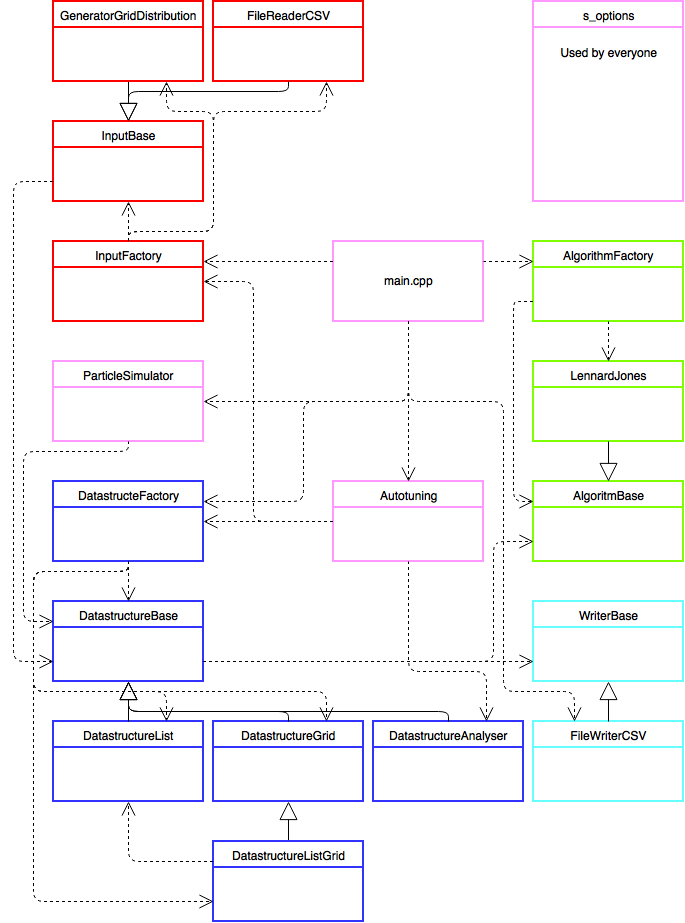
\includegraphics[height=0.6\textheight]{ClassDiagram.png}
		\caption{Klassendiagramm}
		\label{figure:Klassendiagramm}
	\end{figure}
	Das Programm lässt sich grob in 6 Logische Teilbereiche gliedern.\\
	\textbf{Output} (cyan); \textbf{Input} (rot); \textbf{Datenstruktur} (blau); \textbf{Auto-Tuning} (orange); \textbf{Algorithmus} (grün); \textbf{Steuerung} (lila)
	\newpage
	\begin{enumerate}
		\item \textbf{Output}: Damit die Ergebnisse der Simulation später ausgewertet werden können, müssen diese als Datei vorhanden sein, damit andere Programme zur Visualisierung verwendet werden können. Hierfür wurde in diesem Projekt ein Modul implementiert, welches alle Partikel in einer '*.csv' Datei Serie abspeichern kann. Der Grund für die Wahl des Dateiformates besteht darin, dass '*.csv' Dateien von jedem Visualisierungswerkzeug geladen werden können, während Binärformate immer nur von einer Teilmenge der Visualisierungswerkzeug unterstützt werden. Wenn ausschließlich Analysen zur Laufzeit ausgeführt werden sollen, oder es darum geht Laufzeiten zu messen, dann kann der Output auch deaktiviert werden, um die reine Rechenzeit messen zu können.
		\item \textbf{Input}: Damit die Simulation starten kann, müssen Partikel vorhanden sein. Da es verschiedene Möglichkeiten geben soll, wie die Partikel zu beginn der Simulation angeordnet sind, ist hier eine sehr gute Austauschbarkeit von verschiedenen Datenquellen erforderlich. Zum einen können die Partikel zur Laufzeit unter Berücksichtigung von Start Parametern generiert werden, zum anderen können die Partikel auch aus einer Datei geladen werden. Im Rahmen dieses Projekts werden die Partikel ausschließlich aus '*.csv' Dateien geladen. Dies liegt daran, dass dieses Programm auch nur Dateien im '*.csv* Format abspeichern kann. Aufgrund der Schnittstellendefinition wäre es möglich weitere Dateiformate hinzuzufügen, ohne viele andere Klassen ändern zu müssen.
		\item \textbf{Datenstruktur}: Zu beginn des Projektes wurden zwei verschiedene Strategien zur Optimierung vorgeschlagen. Es wurde darauf geachtet, dass die Datenstruktur schnell ausgetauscht werden kann. Dies ist insbesondere für das Auto-Tuning notwendig. Zudem ist es hier wie bei den meisten Komponenten einfach möglich weitere und andere Optimierungen einzufügen. Im Gegensatz zu den anderen Austauschbaren Komponenten, wurden hier mehrere Funktionen in der Basisklasse implementiert. Dies wird insbesondere dadurch ermöglicht, dass die Daten selbst in eine Hilfsklasse gekapselt wurden, um die Kombinierbarkeit verschiedener Datenstrukturen zu ermöglichen.
		\item \textbf{Auto-Tuning}:	Das Auto-Tuning entscheidet zu beginn des Programms, welche optimierte Datenstruktur die Programmlaufzeit am stärksten verkürzen kann. Um nach X Iterationen erneut zu entscheiden, welche Datenstruktur am besten geeignet ist, wäre es möglich die Partikel abzuspeichern, und von dem Speicherstand erneut zu starten. Dies ist ohnehin notwendig, wenn die vom Batchsystem zur Verfügung gestellte Laufzeit nicht ausreichend lang ist.
		\item \textbf{Algorithmus}: Es gibt verschiedene physikalische oder chemische Zusammenhänge zwischen verschiedenen Partikeln oder Molekülen. Da es theoretisch möglich sein soll, dieses Verfahren auch durch Parameter zu ändern, wurde auch hier darauf geachtet, dass der Code so organisiert ist, dass eine einfache Austauschbarkeit erreicht wird. Zusätzlich zur Austauschbarkeit ist die Erweiterbarkeit ebenfalls möglich. Während dieses Projektes wurde ausschließlich das Lennard-Jones Potential zur Kräfteberechnung implementiert. Selbst wenn später andere Algorithmen zur Kraftberechnung verwendet werden, sind die Datenstrukturen mit allen Optimierungen weiterhin verwendbar. Um den Datenstrukturen die Möglichkeit zu geben, Optimierungen anzuwenden wurde der Algorithmus in zwei Teile aufgespalten. Der erste Teil beschränkt sich auf die Bewegung, die aus der aktuellen Geschwindigkeit des einzelnen Partikels resultiert. Der zweite Teil beschränkt sich auf die Kräfte, die durch Wechselwirkungen zwischen Partikeln entstehen.
		\item \textbf{Steuerung}: Ein Teil des Programms ist für die Kontrolle der anderen Teilbereiche zuständig. Zur den Kontrollstrukturen gehören in diesem Programm die Parameter, welche die Startbedingungen definieren, da aufgrund der Parameter völlig unterschiedliche Ergebnisse produziert werden können. Die Partikel Simulator Klasse steuert das Verhalten der verschiedenen Iterationen und führt Aktionen zwischen den Iterationen aus. Unter anderem können die Daten zwischen den Iterationen mithilfe der Output Komponente gespeichert werden.
	\end{enumerate}
	Die vorherigen Aspekte behandelten das Design und die Implementierung der logischen Teilbereiche des Programms. Im folgenden werden weitere wichtige Aspekte beschrieben, die sich nicht in logische Teilbereiche einordnen lassen, sondern allgemein Anwendung finden.
	\begin{itemize}
		\item \textbf{Parameter} Schon zu beginn des Projektes war absehbar, dass das Programm mit verschiedenen Startparametern umgehen können muss. Zum einen ist dies sehr hilfreich, um zum Testen spezielles Verhalten zu provozieren, zum anderen ermöglicht ein parametrisierter Programmaufruf eine sehr flexible Einsatzmöglichkeit des Programms. Während des Programmierens wurden zunehmend mehr Parameter hinzugefügt. Sodass die Art wie die Parameter im Programm abgespeichert werden angepasst werden musste. Sobald die ersten Parameter übernommen werden konnten, war das hinzufügen weiterer Parameter sehr einfach. Um es späteren Anwendern zu erleichtern wurde für jeden Programmparameter ein Hilfetext aufgeschrieben. Der Hilfetext für alle Parameter kann mithilfe des Parameters '-{}-help' ausgegeben werden. Zur Implementierung der Parameter wurde get-opt verwendet, da diese Bibliothek es ermöglicht die Parameter ohne großen Aufwand zu Parsen.
		\item \textbf{Schnittstellen} Da in diesem Projekt an vielen Stellen die Austauschbarkeit gegeben sein muss, wurde als einheitliche Methode für die Austauschbarkeit abstrakte Klassen benutzt. Durch abstrakte Klassen ist es einfach möglich, die Basisklasse durch beliebige abgeleitete Versionen zu ersetzen. Die Schwierigkeit bei den verwendeten Schnittstellen bestand darin eine Menge von Funktionen zu definieren, die für alle Implementationen gleichermaßen sinnvoll sind. Um die volle Flexibilität zu erreichen musste darauf geachtet werden, dass immer nur Funktionen der Basisklasse aufgerufen werden, und niemals spezielle Funktionen einer der Implementationen.
		\item \textbf{Logging} Beim Programmieren ist es manchmal sinnvoll, lokale Variablen auf die Konsole zu schreiben, um den aktuellen Status des Programms zur Laufzeit nachverfolgen zu können. Auch zur Fehlersuche ist dies manchmal sehr hilfreich, da Debugger die Ausführungszeit teilweise so stark verlangsamen, dass einige Fehler dadurch nicht mehr auftreten. Deshalb wurden schon zu beginn des Projekts Funktionen implementiert, welche hilfreiche Informationen ausgegeben können, während das Programm getestet wird. Um dafür zu sorgen, dass die Release-Version nicht unnötig durch Textausgaben verlangsamt wird, wurden Makros verwendet, welche selbst den Funktionsaufruf für die Debug-Ausgaben aus dem Programm entfernen können. Der Grund hierfür ist, dass selbst der Aufruf einer leeren Funktion etwas Zeit kostet. Durch große Anzahlen an Funktionsaufrufen, würde selbst diese Zeit zu merkbare Laufzeitunterschieden führen. Da es häufig vorkommt, dass der selbe Datentyp an verschiedenen Stellen ausgegeben werden soll, wurden die entsprechenden std::stream-Operatoren überschrieben, wodurch auch Vektoren oder ganze Klassen relativ einfach und lesbar in der Log-Datei wiederzufinden sind. Dies erleichtert das Suchen nach Semantik Fehlern in den Debug-Ausgaben in den Log-Dateien.
		\item \textbf{Präzision} Wenn es ausreichend ist, die Partikel mit einfacher Fließkomma Präzision zu berechnen, dann ist es unsinnig, die Partikel Interaktionen mit doppelter Genauigkeit zu berechnen. Um dieses Verhalten ändern zu können wurde ein typedef verwendet, welches diese Genauigkeit festlegt. Dies ermöglicht der Vektorisierung bei ausreichender Partikel Anzahl in der Nachbarschaft, dass doppelt so viele Partikel Interaktionen gleichzeitig berechnet werden.
		\item \textbf{Parameterübergabe} Unter Berücksichtigung der Datenstrukturen, die zur Optimierung verwendet werden sollen, ist es sinnvoll, Teilbereiche von Arrays als Parameter übergeben zu können. Da die entsprechenden Funktionen sehr oft aufgerufen werden, ist es nicht tragbar, die Werte jedes mal zu kopieren. Deshalb werden ein Zeiger auf das erste Element, sowie eine Längenangabe als Parameter übergeben. 
	\end{itemize}
	\section{Korrektheit}%DONE
	Um sicherzustellen, dass das Programm korrekte Ausgaben liefert, wurden verschiedene Arten von Test durchgeführt. Zum einen wurden einzelne Komponenten getestet, zum anderen wurde auch das Gesamtverhalten des Programms überprüft.
	\begin{itemize}
		\item \textbf{Unit-Tests} Um die Korrektheit von den einzelnen Komponenten des Programms zu gewährleisten wurden Unit-Tests eingesetzt. Schon beim Schreiben der Unit-Tests wurden viele Fehler gefunden und behoben. Bei späteren Refactoring-Maßnahmen wurden durch diese Testfälle viele neue Fehler verhindert. Zudem konnten diese Testfälle helfen, wenn neue Implementationen von abstrakten Klassen eingefügt wurden. Hier konnte man die neue Implementierung so lange verbessern, bis die schon existierenden Unit-Tests nicht mehr fehlschlagen.
		\item \textbf{Energieerhaltung} Aus dem Physikalischen Gesetz 'Aktion gleich Reaktion' ergibt sich, dass die Energie in einem geschlossenen System immer erhalten bleiben muss. Eingebaute Funktionen im Programm ermöglichen die Ausgabe der aktuellen Energie im System, sodass leicht überprüft werden kann, ob die Energie in einem akzeptablen Rahmen bleibt. Durch Rechenungenauigkeiten ist es sehr unwahrscheinlich, dass die Energie exakt gleich bleibt.
		\item \textbf{Visualisierung} Durch die Visualisierung der Ausgabedaten wurde auch das Gesamtergebnis stichprobenartig überprüft. Bei den getesteten Parametern verhielt sich das Programm wie erwartet.
	\end{itemize}
	\section{Parallelisierung}%DONE
	Im Verlauf des Projektes wurden die Interaktionen auf Zellenbasis parallelisiert (siehe Figure \ref{figure:OpenMPAufteilung}). Dies liegt daran, dass per Definition nur Partikel in aneinandergrenzenden Zellen interagieren können. Da es sich um kurzreichweitige Partikel Interaktionen handelt, gibt es mit steigender Partikel Anzahl auch mehr Zellen. Hieraus folgt, dass die Parallelisierung viele Möglichkeiten hat, die Last unter den Threads sinnvoll aufzuteilen. Die nur Listen basierende Version wurde nicht parallelisiert, da diese deutlich mehr Laufzeit benötigt um die Datenstruktur zu reorganisieren. 
	\begin{figure}[h]
		\centering
		\includegraphics[width=0.5\textwidth]{LinkedCellsParallel.png}
		\caption{OpenMP Rechenverteilung}
		\label{figure:OpenMPAufteilung}
	\end{figure}\\
	In der Figure \ref{figure:OpenMPAufteilung} kann man sehen, dass ein Thread immer nur einen 2x2x2 Block benötigt, um Interaktionen zu berechnen. Nachdem alle 2x2x2 Blöcke in einem zweier Raster berechnet wurden, ist es notwendig mithilfe von einem Offset dieses zweier Raster zu verschieben, sodass schlussendlich alle Interaktionen betrachtet werden. %absichtlich leere Zeile Folgt
	
	In der Figure \ref{figure:OpenMPSpeedup} ist das Skalierungsverhalten des Programms dargestellt. Mit bis zu 11 Threads ist das Skalierungsverhalten relativ gut. Bei 13 oder mehr Threads muss der Prozessor auf dem zweiten Sockel mit benutzt werden. Dies führt zu deutlich längeren Zugriffszeiten auf den lokalen Speicher des jeweils anderen Prozessors. Hinzu kommt, dass zwar der Laufzeit intensivste Programmteil parallelisiert wurde, aber nicht das gesamte Programm. Dies führt bei insgesamt kürzeren Laufzeiten zu einem immer größeren relativem Anteil des sequentiellen Codes.
	\begin{figure}[h]
		\centering
		\begin{tikzpicture}
		\begin{axis}[
		width=0.7\textwidth,
		xmin = 0,
		xmax = 26,
		xtick = {2,4,6,...,24},
		ymin = 0,
		ymax = 9,
		legend pos=south east,
		xmajorgrids=true,
		ymajorgrids=true,
		grid style=dashed,
		ytick = {0.5,1,...,8.5},
		xlabel = Threads, 
		ylabel = Speedup]
		\addplot table [domain=1:16, samples=1000,x=threads, y=speedup, col sep=comma] {times_openmp_skalierung.csv};
		\end{axis}
		\end{tikzpicture}
		\caption{OpenMP Speedup Diagramm}
		\label{figure:OpenMPSpeedup}
	\end{figure}
	\section{Vektorisierung}
	Bei der Vektorisierung wurde sich auf die Funktionen step\_2(...) und step\_2\_offset(...) konzentriert. Diese Funktionen dienen der Interaktionsberechnung mit Hilfe des Störmer-Verlet-Verfahrens und entsprechen über 90\% der Laufzeit. Diese Laufzeitanteile ergaben Messungen mit Gprof, deren Ergebnisse in der folgenden Tabelle zu sehen sind. 
	\begin{table}[h]
		\centering
		\begin{tabular}{c|l|l}
			\# particles  & step\_2 &  step\_2\_offset \\
			\hline
			32768 & 80.37\% & 16.24\% \\
			\hline
			42875 & 82.62\% & 15.21\%\\
			\hline
			64000 & 85.15\% & 12.91\%\\
		\end{tabular}
		\caption{Laufzeitanteil}
		\label{table:Laufzeitanteil}
	\end{table}\\
	%öäü
	Die Funktionen sind fast identisch mit dem Unterschied, dass step\_2\_offset weitere Parameter besitzt um die Interaktion zwischen zwei an den Rändern positionierten Zellen zu berechnen. Dadurch wurde bei der Vektorisierung für beide Funktionen dasselbe gemacht. Für die Vektorisierung wurde zunächst der in den Funktionen enthaltende if-Block, der nur ausgeführt wird, wenn die gerade zu berechnenden Partikel eine Distanz haben, die kleiner als der cut-off-Radius ist, durch die Abfrage ob der Abstand geringer ist als der cut-off-Radius ersetzt. Das Ergebnis des Vergleiches wird als Initialisierung für die  zu errechnende Kraft der potentiellen Interaktion genutzt. Daraus resultiert, dass die Kraft als null initialisiert wird und somit bei einer Multiplikation mit der Kraft der Interaktion weiterhin null ergibt, welches bewirkt, dass die Positionsänderung null ist. Ist die Distanz kleiner als der cut-off-Radius so wird der Errechnete Wert mit eins multipliziert und so das Ergebnis verwendet. Bei diesem Vorgehen werden allerdings viele Berechnungen durchgeführt die letzten Endes nicht berücksichtigt werden. Trotzdem wird aus den Messungen ein  relevanter Speedup ersichtlich. Zusätzlich erlaubt die Architektur und der verwendete Algorithmus die Verwendung des \_\_restrict\_\_ Keywords, da keiner der Parameter ein Alias oder ein Subarray eines anderen Parameters ist.
	Dies erlaubt der Autovektorisierung die sonst benötigten Sicherheits-Abfragen für Aliase oder Subarrays weg zu lassen was die Vektorisierung für den Compiler erleichtert.\\
	In der folgenden Tabelle werden die unterschiedlichen Laufzeiten von der unoptimierten und der optimierten Funktion step\_2 dargestellt sowie der entstandene Speedup. Die Messungen sind von einer Simulation mit einem Volumen von $60^3$ und einem Cut-Off-Radius von 6.
	\begin{table}[h]
		\centering
		\begin{tabular}{c|l|l|l|l}
			\# Partikel & nicht optimiert (s) & optimiert (s) & Speedup\\
			\hline
			27000 & 74.09 & 53.27 & 1.39 & 0.125\\
			\hline
			32768 &  103.13 & 67.57 & 1.526 & 0.152\\
			\hline
			42875 & 171.85 & 114.38 & 1.502 & 0.198\\
			\hline
			59319 & 331.96& 223.36  & 1,486& 0.274\\
			\hline
			79507 &586.75 & 384.06 & 1.528 & 0.368\\
		\end{tabular}
		\caption{Vektorisierungs Ergebnisse}
		\label{table:VecErg1}
	\end{table}\\
	Anhand der Ergebnisse lässt sich ein vorläufiger durchschnittlicher Speedup von 1.4864 feststellen.	Um zu testen ob die Dichte der Partikel Auswirkungen auf die Ergebnisse der Vektorisierung haben wurden weitere Tests gemacht, wobei das Volumen auf $45^3$ verringert wurde. Diese weitere Laufzeittests mit ergaben die folgenden werte.
	\begin{table}[h]
		\centering
		\begin{tabular}{c|l|l|l|l}
			\# Partikel & nicht optimiert (s) & optimiert (s) & Speedup & Dichte\\
			\hline
			27000 & 114.31 & 93.41 & 1.54 & 0.296\\
			\hline
			32768 &  212 & 121.45 & 1.747 & 0.360\\
			\hline
			42875 & 364.15 & 230.70 & 1.578 & 0.471\\
			\hline
			59319 & 687.17 & 401.41 & 1.69 & 0.652\\
			\hline
			79507 &1235.49 & 757.71 & 1.63 & 0.872\\
		\end{tabular}
		\caption{Vektorisierungs Ergebnisse}
		\label{table:VecErg1}
	\end{table}\\
	Aus diesen Ergebnissen lässt sich sehen, dass wenn die Dichte der Partikel steigt, dies auch den durch die Vektorisierung erreichten Speedup erhöht. Um dies weiter zu überprüfen wurde eine letzte Messung vorgenommen. Bei dieser wurde das Volumen auf $30^3$ verringert.
	\begin{table}[h]
		\centering
		\begin{tabular}{c|l|l|l|l}
			\# Partikel & nicht optimiert (s) & optimiert (s) & Speedup & Dichte\\
			\hline
			27000 & 386.70 & 201.86 & 1.965 & 1.0\\
			\hline
			32768 &  600.32 & 323.27 & 1.857 & 1.213\\
			\hline
			42875 & 974.18 & 531.70 & 1.834 & 1.588\\
			\hline
		\end{tabular}
		\caption{Vektorisierungs Ergebnisse}
		\label{table:VecErg1}
	\end{table}\\
	Das Ergebnis zeigt noch deutlicher, dass mit der Dichte und somit der steigenden Partikelinteraktionen auch die Effektivitaet der Vektorisierung steigt.
	\newpage
	\section{Auto-tuning}%DONE
	Um herauszufinden, nach welchen Kriterien das Auto-tuning entscheiden kann, wurden viele Messungen mit verschiedenen Parametern durchgeführt. Die Laufzeit des Programmes steigt mindestens Linear mit der Anzahl der zu simulierenden Partikel. Bei kurzreichweitigen Interaktionen kann die Laufzeitabschätzung mit $p\cdot\frac{r^3}{V}\sim O\left(1\right)$ vereinfacht werden (siehe Tabelle \ref{table:Laufzeitvergleich}).\\
	\begin{table}[h]
		\centering
		\begin{tabular}{c|l|l|l|l}
			&Basic& Nachbar-Listen & Linked-Cells & Kombination \\
			\hline
			\begin{tabular}{@{}c@{}}Aufbau \\ (Linked-Cells)\end{tabular} &-& - & $\Theta\left(p\right)$& $\Theta\left(p\right)$\\
			\hline
			\begin{tabular}{@{}c@{}}Aufbau \\ (Nachbar-Listen)\end{tabular}&-& $\Theta\left(p^2\right)$ & - & \begin{tabular}{@{}l@{}}$O\left(p^2\cdot \frac{27 \cdot r^3}{V}\right)$ \\ $\sim O\left(p\cdot 27\right)$\end{tabular} \\
			\hline
			Iteration& $\Theta\left(p^2\right)$&\begin{tabular}{@{}l@{}}$O\left(p^2\cdot \frac{\frac{4}{3}\pi\cdot r^3}{V}\right)$\\$\sim O\left(p\cdot \frac{4}{3}\pi\right)$\end{tabular} &\begin{tabular}{@{}l@{}}$O\left(p^2\cdot \frac{27 \cdot r^3}{V}\right)$\\$\sim O\left(p\cdot 27\right)$ \end{tabular}& \begin{tabular}{@{}l@{}}$O\left(p^2\cdot \frac{\frac{4}{3}\pi\cdot r^3}{V}\right)$\\$\sim O\left(p\cdot \frac{4}{3}\pi\right)$ \end{tabular}\\
		\end{tabular}
		\caption{Laufzeitvergleich der Datenstrukturen}
		\label{table:Laufzeitvergleich}
	\end{table}\\
	\footnotesize\textbf{Abkürzungen:}\begin{labeling}[~--]{MAX}
		\item[p] Partikel Anzahl
		\item[r] cut-off-Radius
		\item[V] gesamt Volumen
	\end{labeling}
	Die Gesamtlaufzeit hängt von den Faktoren 'Wie oft wird die Datenstruktur neu organisiert?' und 'Wie lange dauert das Umorganisieren?' ab. 
	\newpage
	\subsection{Wie oft wird die Datenstruktur neu organisiert?}%DONE
	Wie oft die Datenstruktur neu organisiert werden muss hängt von den folgenden Eingabeparametern in deren Kombination ab.
	\begin{itemize}
		\item \textbf{cut-off Zusatzbereich} Je mehr Spielraum auf den cut-off-Radius hinzugefügt wird, desto seltener müssen die Datenstrukturen neu aufgebaut werden. Dies geht allerdings auch sehr zulasten der Laufzeit, die in den Iterationen gebraucht wird.
		\item \textbf{Startgeschwindigkeit} Je schneller sich die Partikel sich bewegen, desto schneller wird der dem cut-off-Radius hinzugefügte Bereich verlassen. Hieraus folgt, dass die Datenstruktur häufiger neu aufgebaut werden muss.
		\item \textbf{Maximale Iterationen ohne Reorganisation} Manchmal ist es sinnvoll anzugeben wie oft die Datenstruktur mindestens neu gebaut werden muss. Dies ist insbesondere dann sinnvoll, wenn die Startgeschwindigkeit 0 ist.
	\end{itemize}
	\begin{align*}
	r \cdot (f - 1)&=i\cdot v\\
	\frac{r \cdot (f - 1)}{v}&=i
	\end{align*}
	\footnotesize\textbf{Abkürzungen:}\begin{labeling}[~--]{MAX}
		\item[r] cut-off-Radius
		\item[f] cut-off-Radius-Faktor
		\item[v] Startgeschwindigkeit
		\item[i] Iterationen
	\end{labeling}
	Strecke ist gleich Zeit multipliziert mit Geschwindigkeit - das ist die Grundidee hinter der Formel die berechnet, wie oft die Datenstruktur neu gebaut werden muss. Zwei der Variablen, Geschwindigkeit und Strecke, sind zu beginn des Programms gegeben. Mit Strecke ist hier die Distanz gemeint, die maximal zurückgelegt werden darf bevor die Datenstruktur neu gebaut werden muss.
	\subsection{Wie lange dauert das Reorganisieren der Datenstrukturen?}%DONE
	Wie lange dauert es die Datenstruktur neu zu bauen? Wie viel schneller wird durch den Mehraufwand des Neubauens die einzelne Iteration? Je nachdem, welches Verfahren gewählt wird, ist die Laufzeit unterschiedlich. Bei der Variante welche nur Nachbar-Listen verwendet, steigt der Aufwand diese Listen aufzubauen quadratisch zur Anzahl der Partikel. Dies ist so ungünstig, dass es nicht empfehlenswert ist, diese Variante zu benutzen. Die Nachbarschaftslistenvariante benötigt wenig Zeit um die Datenstruktur aufzubauen, dafür aber wird pro Iteration viel Zeit benötigt. Die kombinierte Variante benötigt mittelmäßig viel Zeit für den Aufbau der Datenstruktur, und nur Minimale Zeit pro Iteration. Auch die Laufzeit für das Neubauen hängt von verschiedenen Parametern ab.
	\begin{itemize}
		\item \textbf{cut-off Radius} Je größer der cut-off- Radius gewählt wird, desto mehr Partikel befinden sich in der Nachbarschaft. Die Zellen werden hierdurch größer. Wenn der cut-off- Radius relativ groß ist, dann ist die Laufzeit pro Iteration in der nur Zellen basierten Version länger, in der kombinierten Variante hingegen steigt die benötigte Laufzeit für den Neuaufbau der Datenstruktur. Allgemein gilt, je mehr Partikel in einer Zelle sind, desto günstiger wird die Verwendung der kombinierten Variante, solange diese nicht allzu häufig neugebaut werden muss. Da dieses Programm sich auf kurzreichweitige Interaktionen fokussiert, werden keine sehr großen cut-off- Radien auftreten.
		\item \textbf{Dichte} Wenn die Partikel dichter aneinander liegen, führt das dazu, dass sich Potentiell mehr Partikel innerhalb des cut-off- Radius befinden.
		\item \textbf{Partikel Anzahl} Wenn die Anzahl der Partikel sehr gering ist, dann ist die Laufzeit des naiven Algorithmus ohne Optimierung kürzer, als eine der Optimierten Varianten, da der Naive Algorithmus nur sehr kleine Konstanten hat. Sobald mehrere hundert Partikel verwendet werden lohnt es sich optimierte Datenstrukturen zu verwenden, um unnötige Interaktionen schnell herausfiltern zu können. Wenn die absolute Anzahl der Partikel sehr groß ist, dann lohnt sich jedes einzelne Partikelpaar zwischen dem keine Interaktion berechnet werden muss. Die Listen basierenden Verfahren reduzieren die Laufzeit pro Iteration auf ein Minimum, haben aber einen dementsprechend größeren Zeitaufwand beim Neubauen der Datenstruktur. 
		\item \textbf{Startanordnung} Je nachdem wie die Partikel bei Programmstart angeordnet sind ergeben sich andere Effekte. Zum Beispiel wäre es möglich, dass sich zu beginn alle Partikel in einem kleinem Bereich des zu simulierenden Raum aufhalten. Hieraus folgt, dass einige Zellen sehr viel mehr Partikel enthalten als andere. In der aktuellen Version des Programms wird für das Auto-Tuning angenommen, das die Partikel einigermaßen gleichmäßig auf das Volumen verteilt sind.
	\end{itemize}
	\begin{figure}[h]
		\centering
		\begin{tikzpicture}
		\begin{axis}[
		width=\textwidth,
		height=0.3\textheight,
		xmin = 0,
		xmax = 27,
		ymin = -1,
		ymax = 5,
		legend pos=north east,
		xmajorgrids=true,
		ymajorgrids=true,
		grid style=dashed,
		ytick = {0,0.5,...,4.5},
		xlabel = cut-off-Radius, 
		ylabel = Quotient/Iterationen,
		xtick = {4,5,6,8,10,12,14,16,18,20,22,24,26},]
		\addplot table [domain=1:16, samples=1000,x=radius, y=fn_s, col sep=comma] {times_rebuild.csv};
		\addlegendentry{$\frac{cn}{mn}$}
		\addplot table [domain=1:16, samples=1000,x=radius, y=fr_s, col sep=comma] {times_rebuild.csv};
		\addlegendentry{$\frac{cr}{mr}$}
		\addplot table [domain=1:16, samples=1000,x=radius, y=iterations_until_mix_is_better, col sep=comma] {times_rebuild.csv};
		\addlegendentry{$\frac{cr-mr}{mn-cn}$}
		\end{axis}
		\end{tikzpicture}
		\caption{Laufzeit-Quotient der verschiedenen Verfahren}
		\label{figure:LaufzeitQuotient}
	\end{figure}
	\footnotesize\textbf{Abkürzungen:}\begin{labeling}[~--]{MAX}
		\item[cn] Zellen Variante Iteration ohne Neubauen
		\item[mn] Misch Variante Iteration ohne Neubauen
		\item[cr] Zellen Variante Iteration mit Neubauen
		\item[mr] Misch Variante Iteration mit Neubauen
	\end{labeling}
	In dem Diagramm (siehe Figure \ref{figure:LaufzeitQuotient}) kann man erkennen, wie sich die Laufzeit relativ verhält, wenn man die verschiedenen Datenstrukturen wählt. Zur Erstellung der Messdaten wurde ein Volumen mit den Abmessungen 100x100x100  betrachtet. Die gemessenen Werte repräsentieren das gesamte Spektrum der verschieden lang reichweitigen Interaktionen. Cut-off-Radien größer als 26 müssen nicht betrachtet werden, da Implementationsabhängig immer mindestens 9 Zellen (als 3x3x3 Würfel) existieren müssen. Dies führt dazu, dass in den Iterationen alle Paare von Partikeln miteinander interagieren. Bei den Iterationen, in denen die Datenstruktur neu gebaut wird, benötigt die kombinierte Datenstruktur immer (genau) doppelt so viel Zeit, wie die nur Zellen basierte Variante. In den Iterationen, in denen kein Neubauen erforderlich wird, ist das Ergebnis nicht mehr ganz so deutlich.
	\begin{align*}
	cr+i\cdot cn&=mr+i\cdot mn\\
	i\cdot mn-i\cdot cn&=cr-mr\\
	i\cdot (mn-cn)&=cr-mr\\
	i&=\frac{cr-mr}{mn-cn}
	\end{align*}
	Die Formel $i=\frac{cr-mr}{mn-cn}$ beschreibt den Zeitpunkt, an dem beide Varianten gleich schnell sind. Durch '$<$' bzw. '$>$' kann entschieden werden, welches Verfahren danach schneller ist. Je nachdem wie genau die Zellgröße dem angegebenen cut-off-Radius entspricht kann der Quotient $i$ stark variieren. An der Figure \ref{figure:LaufzeitQuotient}) kann man erkennen, dass durchschnittlich nach 2 Iterationen die kombinierte Variante schneller ist, als die nur Zellen basierte Variante.
	\subsection{Resultierende Formel}%DONE
	\begin{align*}
	i&=\frac{r \cdot (f - 1)}{v} &\text{'Wie oft?'}\\
	i&>\frac{cr-mr}{mn-cn}\sim 2&\text{'Wie lange?'}\\
	2&<\frac{r \cdot (f - 1)}{s}
	\end{align*}
	\footnotesize\textbf{Abkürzungen:}\begin{labeling}[~--]{MAX}
		\item[r] cut-off-Radius
		\item[f] cut-off-Radius-Faktor
		\item[v] Startgeschwindigkeit
		\item[i] Iterationen
		\item[cn] Zellen Variante Iteration ohne Neubauen
		\item[mn] Misch Variante Iteration ohne Neubauen
		\item[cr] Zellen Variante Iteration mit Neubauen
		\item[mr] Misch Variante Iteration mit Neubauen
	\end{labeling}
	
	\begin{itemize}
		\item \textbf{true} $\rightarrow$ Linked-Cells+Verlet-Listen
		\item \textbf{false} $\rightarrow$ Linked-Cells
	\end{itemize}
	Nachdem aus den vorherigen Kapiteln bekannt ist, wie oft die Datenstruktur neu gebaut werden muss, kann diese Erkenntnis mit dem Verhältnis aus der Dauer des Neubauens kombiniert werden. Die Gleichung, welche die Dauer des Neubauens beschreibt, wurde durch eine Ungleichung ersetzt, welche nicht beschreibt, wann beide Verfahren gleich gut sind, sondern wann das eine Verfahren besser wird. Hierdurch wird eine Ja-Nein Entscheidung möglich.
	
	\chapter{Zusammenfassung}
	\label{Zusammenfassung}
	
	%TODO 
	%partikel sim geschrieben
	%autotuning geschrieben
	%relevante parameter fuer autotuning ermittelt <name paramteres>
	%Optimierung des programes
	
	
	
	\bibliography{literatur}
	\bibliographystyle{ieeetr}
	
	\chapter{Anhang}
	\label{Anhang}
	Verwendete Bibliotheken und Programme zum ausführen des Programms
	\begin{itemize}
		\item Boost
		\begin{itemize}
			\item Unit-Tests
		\end{itemize}
		\item CMake 
		\item Make
		\item clang-format
		\begin{itemize}
			\item automatisches formatieren des Codes
		\end{itemize}
		\item paraview
		\begin{itemize}
			\item Visualisierung der Ausgabe
		\end{itemize}
		\item lcov
		\begin{itemize}
			\item Testabdeckung ermitteln und visualisieren
		\end{itemize}
		\item slurm
		\begin{itemize}
			\item Messtabellen berechnen
		\end{itemize}
		\item doxygen
		\begin{itemize}
			\item Dokumentation des Quelltextes
		\end{itemize}
		\item \LaTeX
		\begin{itemize}
			\item dieses Dokument
			\item Präsentationen
		\end{itemize}
	\end{itemize}
	Verwendete Compiler
	\begin{itemize}
		\item clang-omp -{}-version\\clang version 3.5.0 \\Target: x86\_64-apple-darwin16.4.0\\Thread model: posix	
		\item g++ --version\\g++ (Ubuntu 6.2.0-5ubuntu12) 6.2.0 20161005
		\item g++ --version\\g++ (GCC) 6.3.0\\Ubuntu 16.04.2 LTS\\(cluster)
		%TODO compiler mit denen getestet wurde ergänzen
	\end{itemize}
	
	
	
	
\end{document}